\section{Introduzione}
\subsection{Contesto Applicativo}
\begin{frame}{Convenzione}
\vskip2ex
... un accordo fra l'Università, rappresentata da un docente, ed una azienda, per la realizzazione di un prodotto.
\vskip2ex

le fasi :\\
\vskip2ex
  \begin{enumerate}
    \item Il docente si accorda con un'azienda riguardo ad un progetto.
    \item Il docente, insieme al RAS, valuta i costi e stila la Tabella di Ripartizione dei compensi.
    \item Il RAS prepara un documento da discutere nel prossimo Consiglio di Dipartimento, che deciderà se approvare o meno la convenzione.
    \item In caso di approvazione la convenzione viene \textbf{inserita nell'applicazione}.
    \item ...
    \item La convenzione risulta esaurita (l'importo stabilito è stato pagato interamente) .
  \end{enumerate}
\end{frame}

\begin{frame}{Gestione di una Convenzione}
 \vskip-3ex
 L'applicazione deve \textbf{monitorare} la convenzione dal suo inserimento fino a quando risulti esaurita. 
 \vskip5ex
 In questo intervallo di tempo l'applicazione deve consentire di \textbf{compiere delle operazioni} sulla convenzione.
\end{frame}

\subsection{Requisiti}
\begin{frame}{Requisiti principali}
  \vskip-3ex
  L'applicazione deve consentire di:\\
  \vskip3ex
  \begin{itemize}
   \item inserire convenzioni
   \item inserire rate per una convenzione
   \item visualizzare le convenzioni inserite
   \item aggiornare i dati di una convenzione
   \item notificare le scadenze
  \end{itemize}

\end{frame}

\section{Analisi}
  \begin{frame}{Agenti}
    \vskip-3ex
    \begin{itemize}
     \item L'Operatore:\\
     \vskip3ex
      \begin{itemize}
       \item inserisce, modifica convenzioni
       \item inserisce le rate
      \end{itemize}
     \vskip3ex
     \item Il Docente:\\
      \begin{itemize}
       \item visualizza lo stato delle proprie convenzioni
      \end{itemize}
     \vskip3ex
     \item Il Tempo:\\
      \begin{itemize}
       \item notifica le scadenze
      \end{itemize}

    \end{itemize}

    
  \end{frame}

  \subsection{Casi d'Uso}
  \begin{frame}{Casi d'uso dell'Operatore}
    \begin{figure}[h]
    \label{use_case_diag_operator}
    \centering
    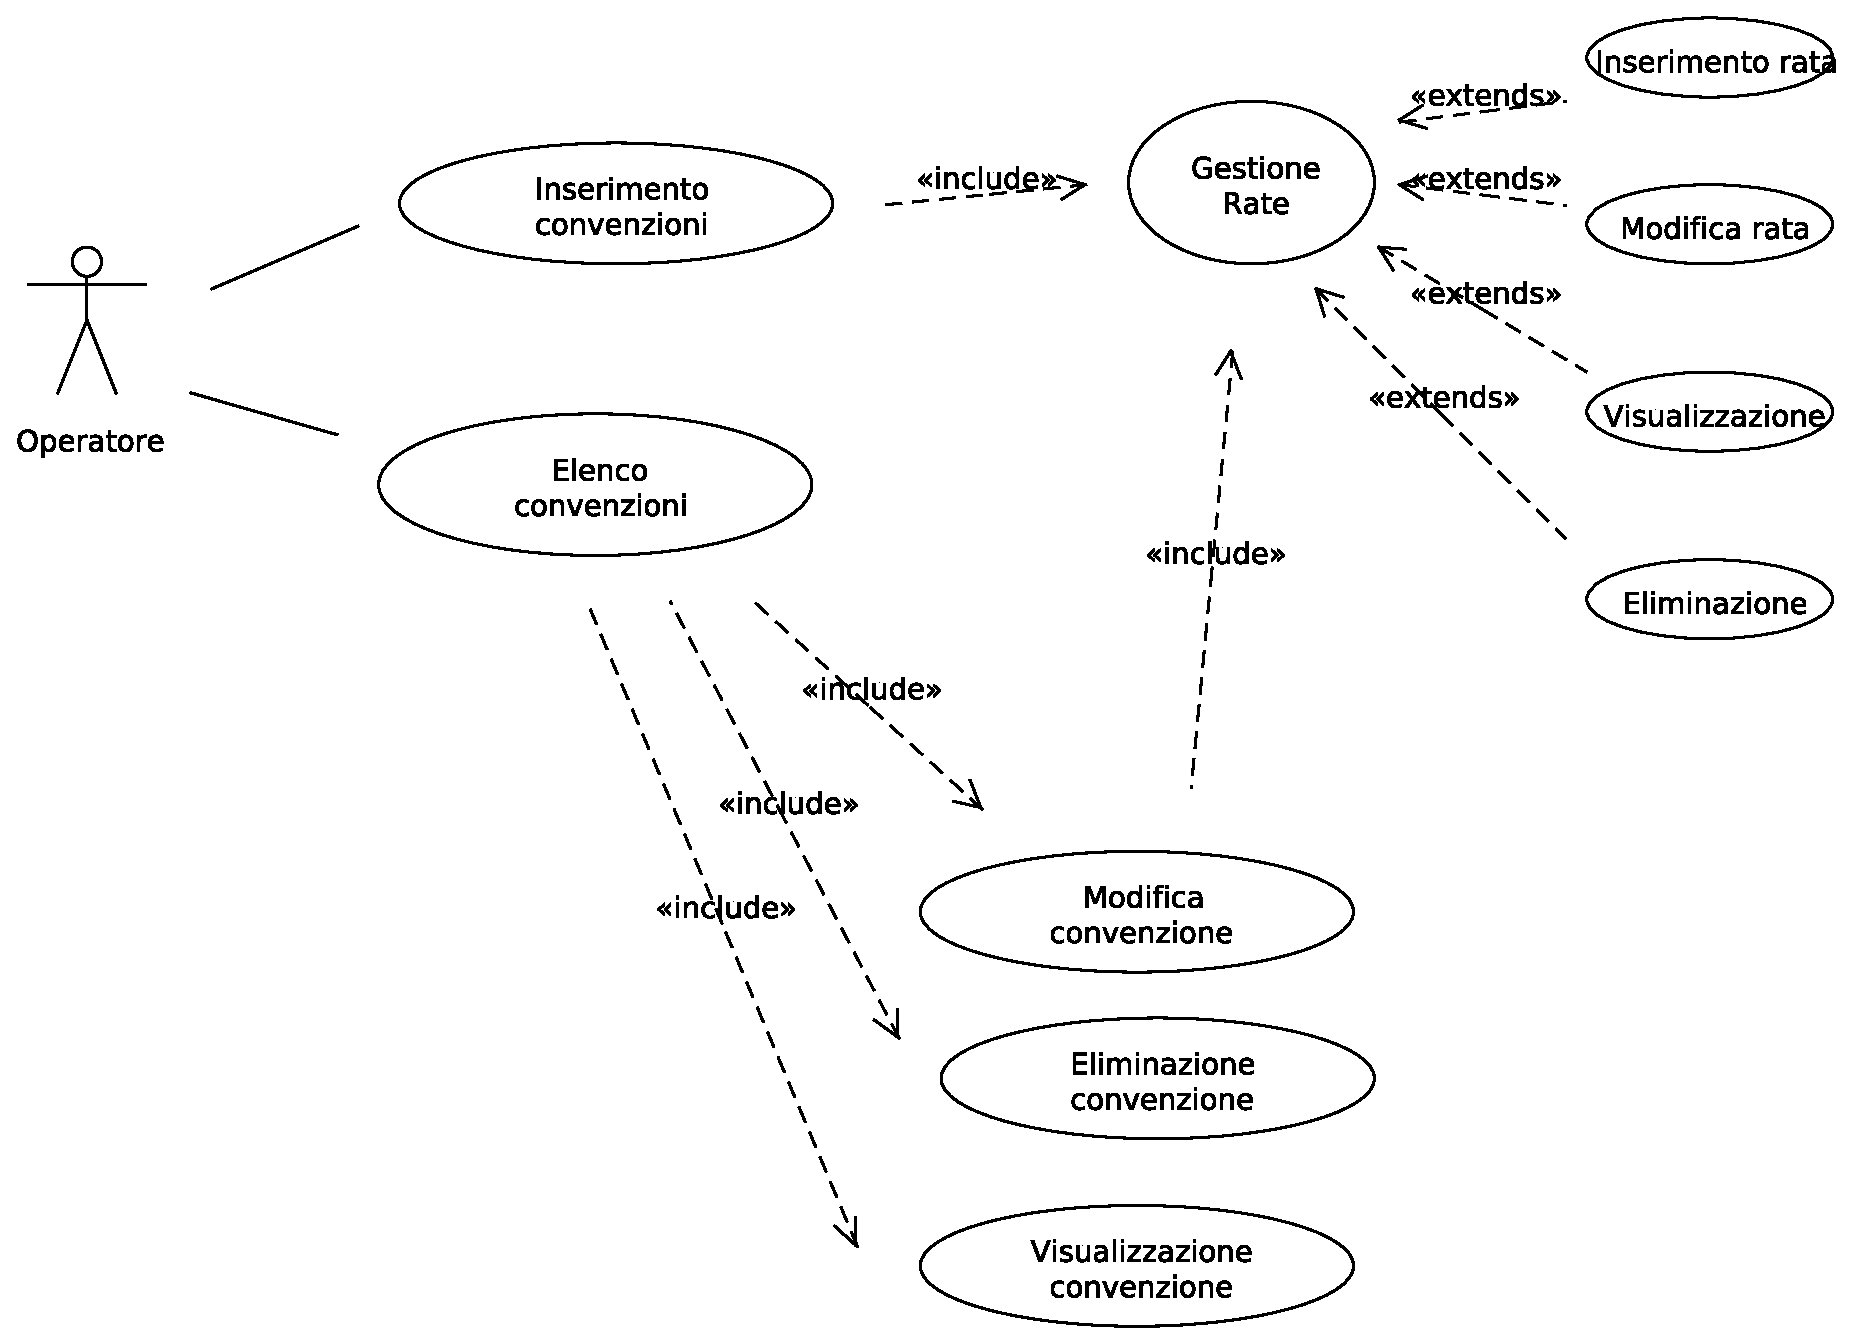
\includegraphics[height=0.8\textheight, width=0.7\textwidth]{images/casi_uso_operatore_semplified.eps}
    \end{figure}
  \end{frame}
  
  \begin{frame}{Esempio di caso d'uso}
   
   \vskip-2ex
      \begin{beamerboxesrounded}[lower=lowercolor, shadow=true]{}
     \begin{center}
	\normalsize{Inserimento di una nuova convenzione\\}
     \end{center}
    \end{beamerboxesrounded}
  
  \vskip2ex
  \textbf{Percorso base}:
  l'Operatore, una volta effettuato il login, clicca su ``Crea una convenzione"; viene visualizzata una schermata suddivisa in varie schede,
  ognuna corrispondente ad un passo della procedura. I passi sono:
  \begin{enumerate}
    \item Inserimento dei dati della convenzione\\
      \begin{itemize}
	\item Il titolo
	\item L'importo totale
	\item ...
      \end{itemize}
            
    \item Inserimento della tabella di ripartizione\\
    \item Inserimento delle rate  
    \item Inserimento della documentazione relativa alla convenzione\\
    \vskip2ex
    
    L'Operatore clicca su ``Salva," la convenzione viene salvata e la procedura termina. Si ritorna alla schermata precedente.
    
  \end{enumerate}
  \end{frame}
  
  \begin{frame}{Esempio di caso d'uso}
  

  \textbf{Percorso alternativo 1}:
  l'Operatore clicca sul tasto ``Salva'' o ``Successivo'' senza aver compilato alcuni dei campi obbligatori, o avendo inserito dei valori non consentiti; viene visualizzato un messaggio di errore 
  e il documento non viene salvato. La schermata non viene cambiata, dando la possibilità all'Operatore di procedere alla correzione.

  
  \vskip3ex
  
  \textbf{Percorso alternativo 2}:
  durante uno qualsiasi dei passi, l'Operatore  clicca sul tasto ``Annulla'', che comporta, a seguito di una conferma, il ritorno alla schermata precedente
  senza che la convenzione venga inserita o i cambiamenti effettuati salvati.
  

   
   
  \end{frame}
  
  \begin{frame}{}
     \begin{figure}[h]
      \centering
      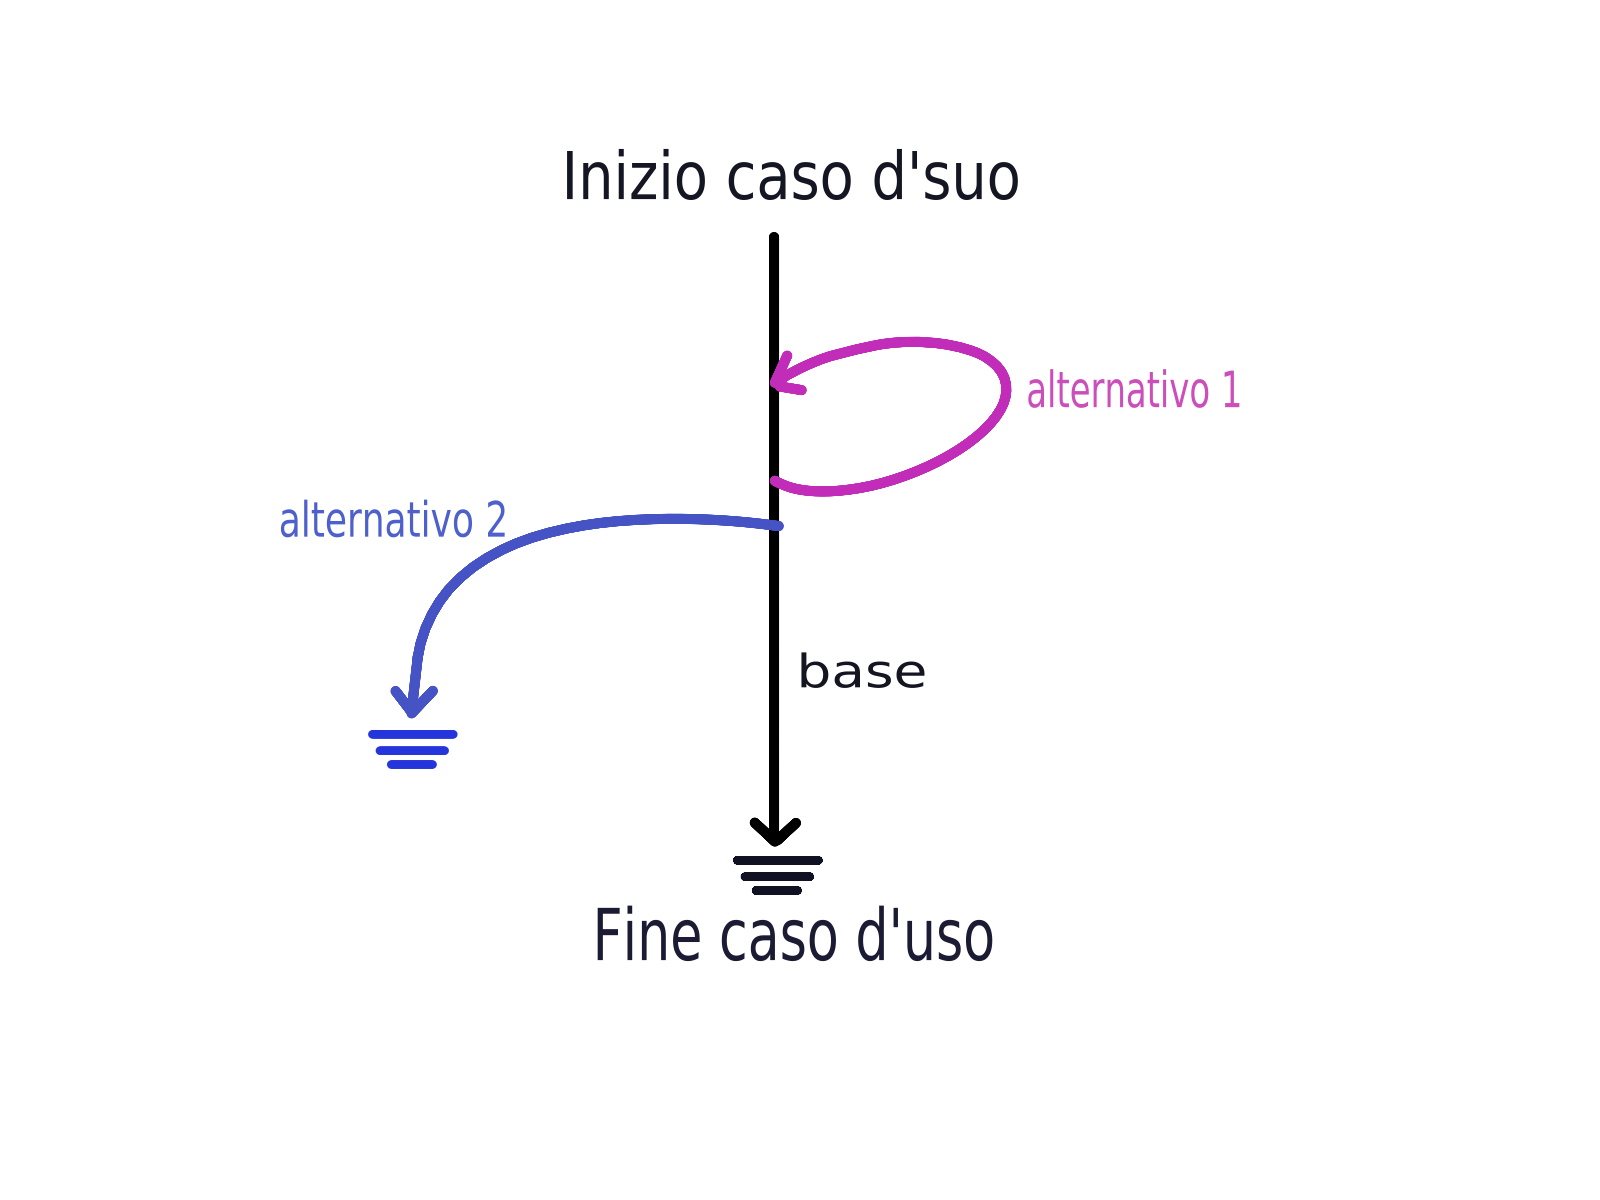
\includegraphics[scale=0.25]{images/flows.png}
    \end{figure}
   
  \end{frame}


  
  \begin{frame}{Casi d'uso del Docente}
    \begin{figure}[h]
      \label{use_case_diag_teacher}
      \centering
      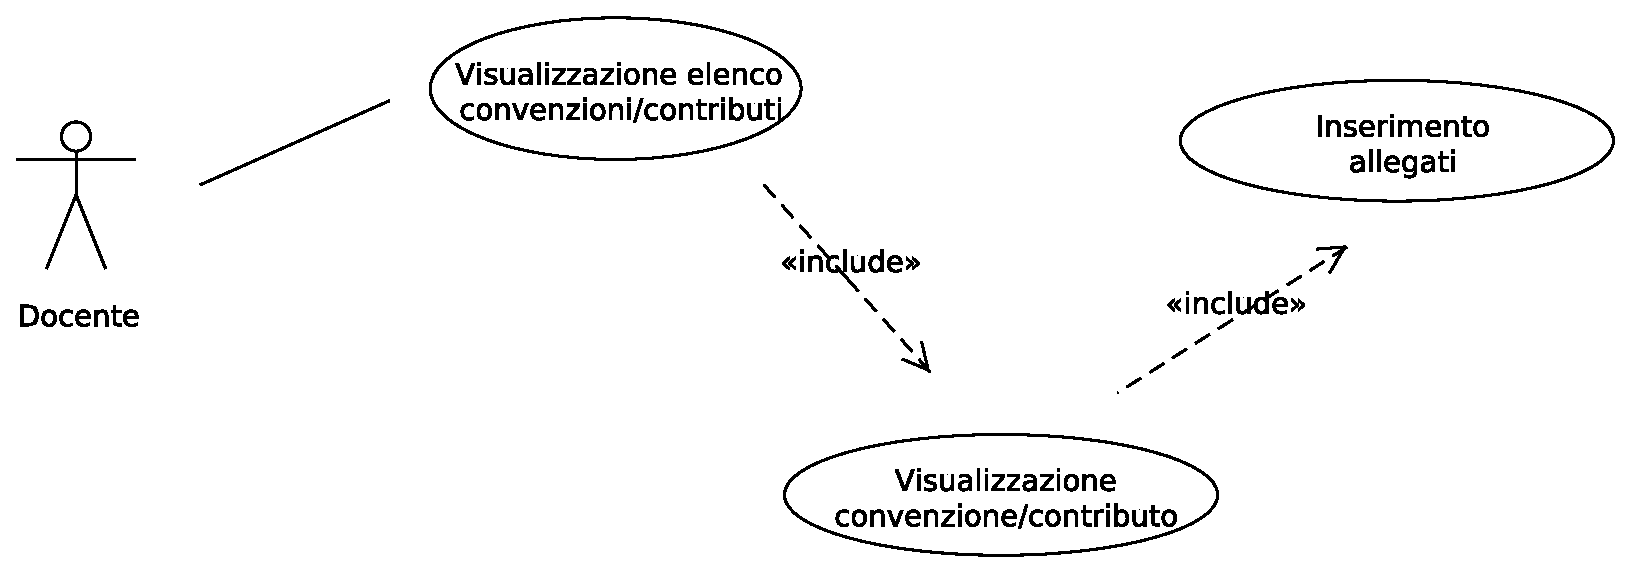
\includegraphics[width=0.8\textwidth]{images/casi_uso_docente.eps}
    \end{figure}
  \end{frame}
  
  \begin{frame}{Casi d'uso del Tempo}
    \begin{figure}[h]
      \label{use_case_diag_time}
      \centering
      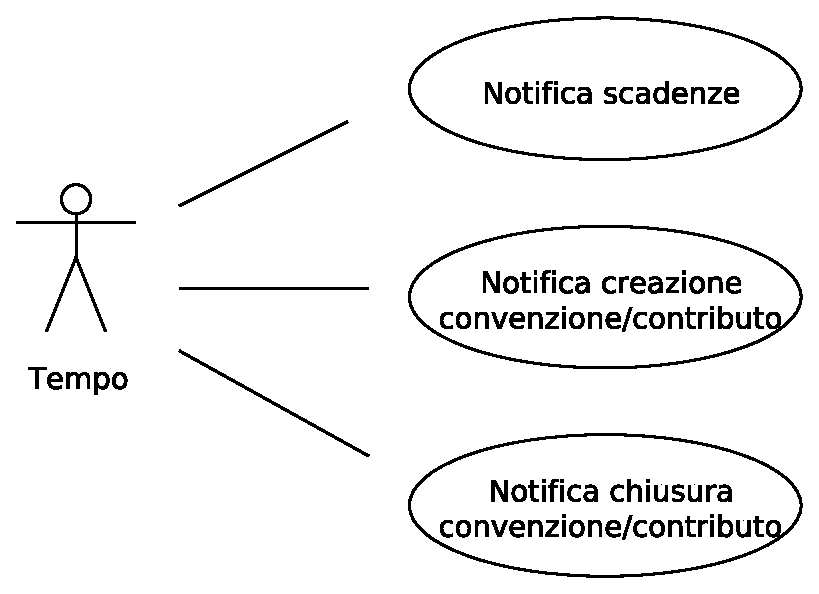
\includegraphics[width = 0.5\textwidth]{images/casi_uso_tempo.eps}
    \end{figure}
  \end{frame}


  
  \subsection{Modello di Business}
  \begin{frame}{Gli oggetti del modello}
     \begin{itemize}
      \item Convenzione
      \item Rata
      \item Responsabile Scientifico
      \item Ditta
      \item ...
     \end{itemize}

   
  \end{frame}
  
  \begin{frame}{Diagramma delle classi}
  
    \begin{figure}[h]
      \label{business_model}
      \centering
      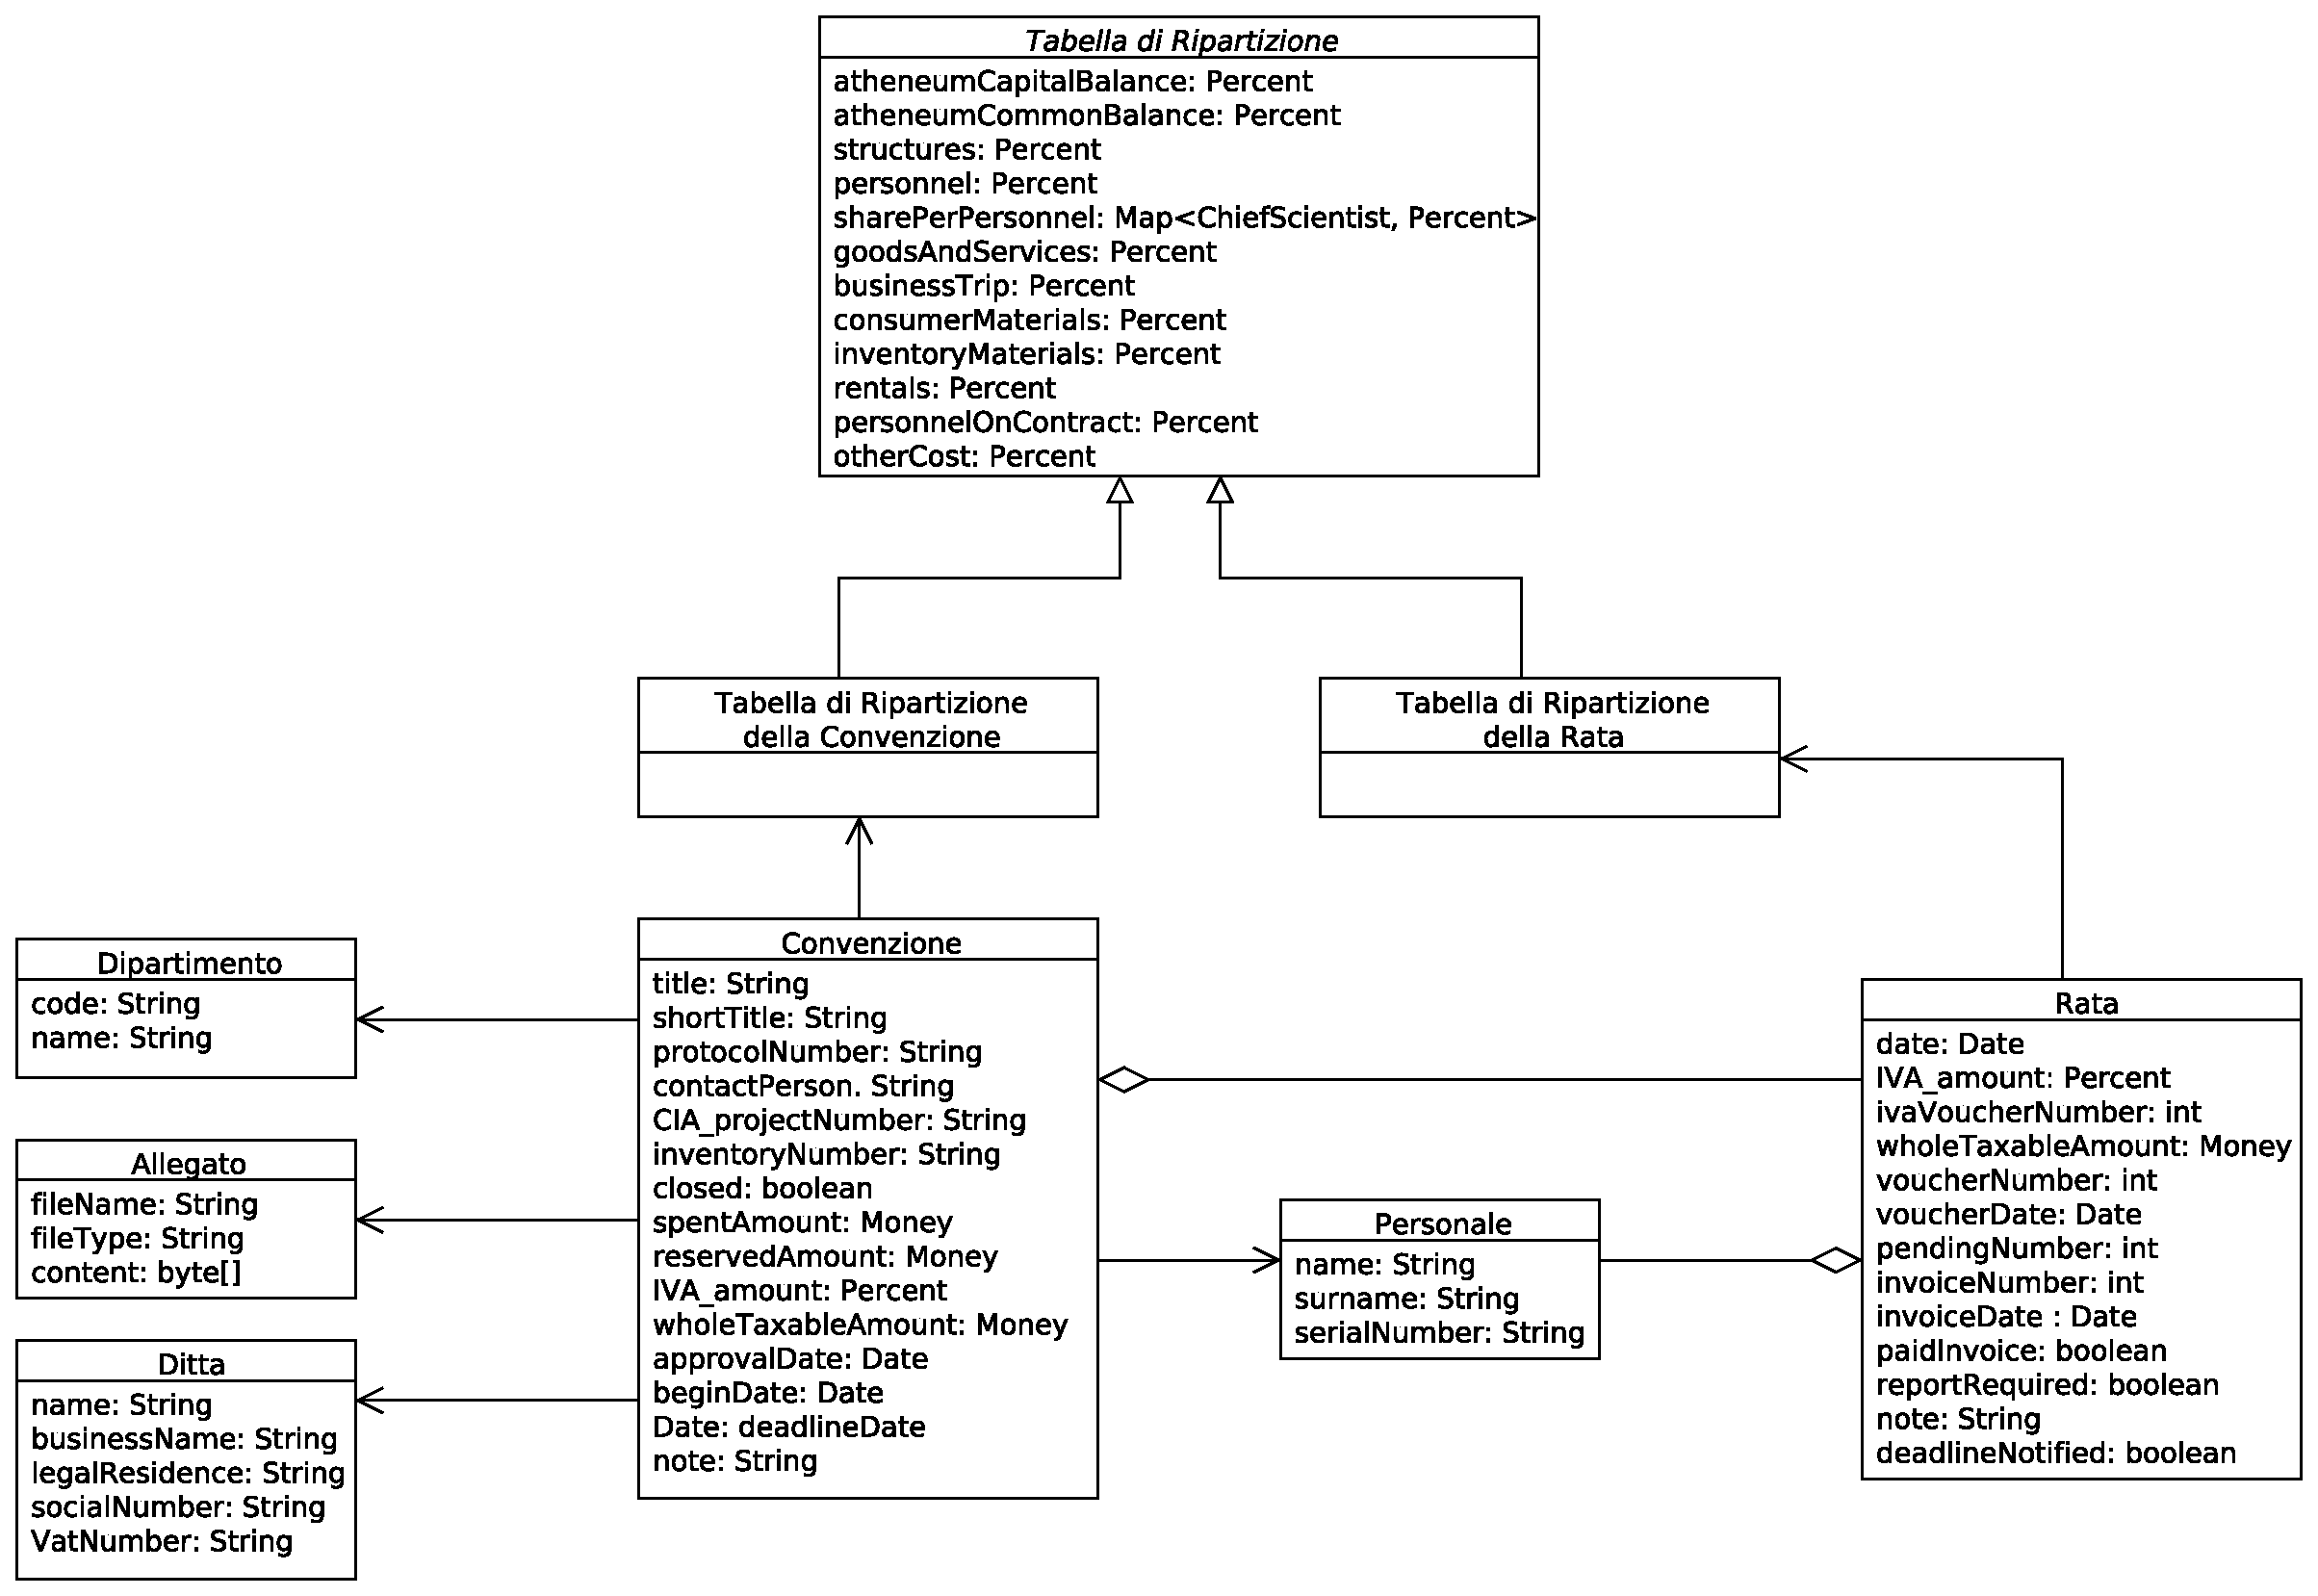
\includegraphics[width=0.8\textwidth]{images/modello_business_simplified.eps}
    \end{figure}
   
  \end{frame}


  
  



